
\begin{frame}
\frametitle{Plagio}
\Huge
\begin{center}
Se buscan integrantes para ingresar al Salon de la fama del PLAGIO
\end{center}
\end{frame}

\begin{frame}
\frametitle{Plagio}

\begin{columns}[c] % The "c" option specifies centered vertical alignment while the "t" option is used for top vertical alignment
\column{.68\textwidth} % Left column and width
\begin{itemize}
\item Reprobación automática a quien reproduzca códigos de otros compañeros y los reporte como suyos, ademas de una nota en su expediente con copia para el consejo de calidad 
\end{itemize}
\column{.28\textwidth} % Left column and width
\begin{center}

\includegraphics[scale=0.27]{Plagio/tarjeta-roja.jpg}
\end{center}
\end{columns}
\begin{center}
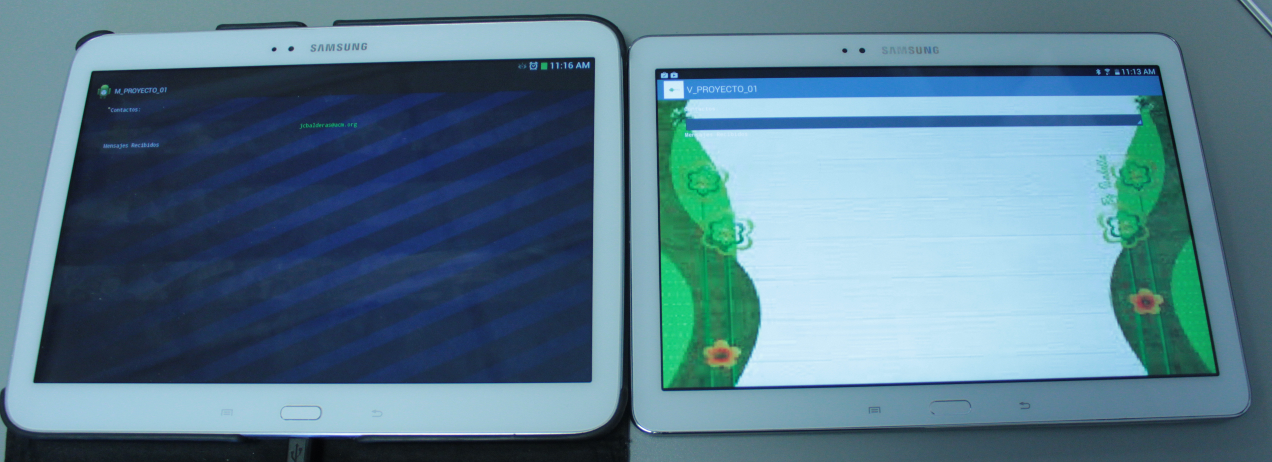
\includegraphics[scale=0.23]{Plagio/Pirata01}
\end{center}
\end{frame}


\begin{frame}
\frametitle{Plagio}
\begin{columns}[c] % The "c" option specifies centered vertical alignment while the "t" option is used for top vertical alignment
\column{.68\textwidth} % Left column and width
\begin{itemize}
\item Reprobación automática a quien copie códigos de Internet y los reporte como suyos, ademas de una nota en su expediente con copia para el consejo de calidad 
\end{itemize}
\column{.28\textwidth} % Left column and width
\begin{center}

\includegraphics[scale=0.27]{Plagio/tarjeta-roja.jpg}
\end{center}
\end{columns}
\begin{center}
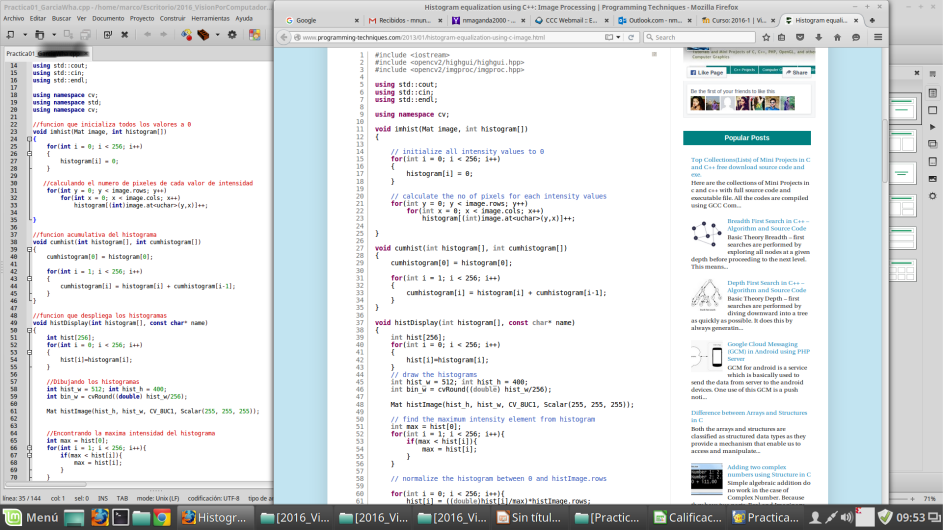
\includegraphics[scale=0.23]{Plagio/Pifia}
\end{center}
\end{frame}

\begin{frame}
\frametitle{Plagio}
\begin{columns}[c] % The "c" option specifies centered vertical alignment while the "t" option is used for top vertical alignment
\column{.68\textwidth} % Left column and width
\begin{itemize}
\item Reprobación automática a quien copie códigos de Internet y los reporte como suyos, ademas de una nota en su expediente con copia para el consejo de calidad 
\end{itemize}
\column{.28\textwidth} % Left column and width
\begin{center}

\includegraphics[scale=0.27]{Plagio/tarjeta-roja.jpg}
\end{center}
\end{columns}
%\url{https://github.com/naman14/AlgorithmVisualizer-Android}
\href{https://github.com/naman14/AlgorithmVisualizer-Android}{https://github.com/naman14/AlgorithmVisualizer-Android}

\begin{columns}[c] % The "c" option specifies centered vertical alignment while the "t" option is used for top vertical alignment
\column{.44\textwidth} % Left column and width
\begin{center}
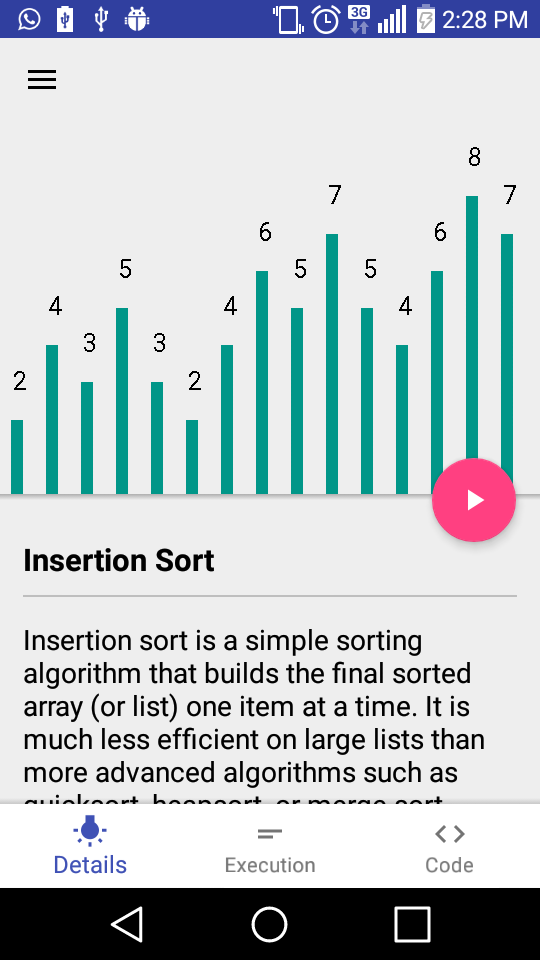
\includegraphics[width=2.3cm]{Plagio/Piratazo_Orig1}\hspace{0.05cm}
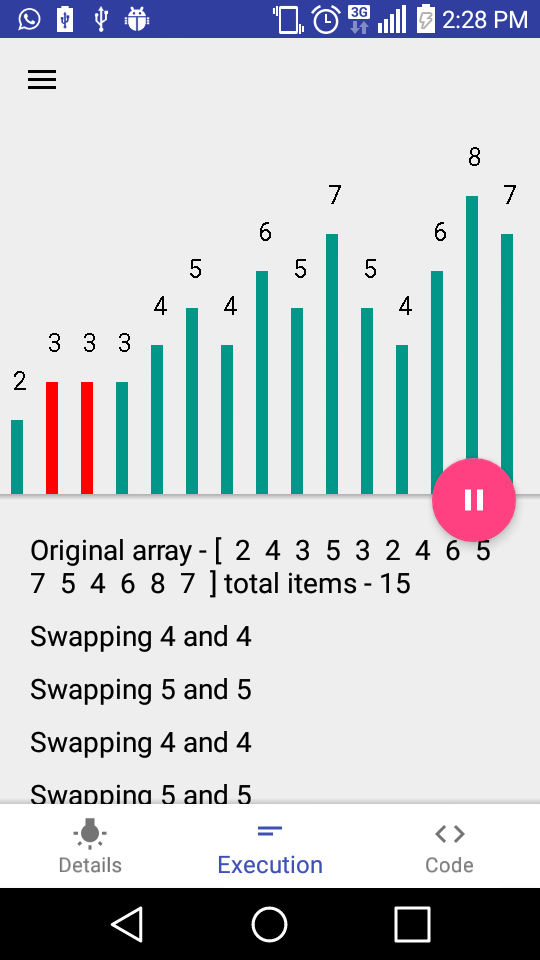
\includegraphics[width=2.3cm]{Plagio/Piratazo_Orig2}\\
Proyecto Original
\end{center}
\column{.44\textwidth} % Left column and width
\begin{center}
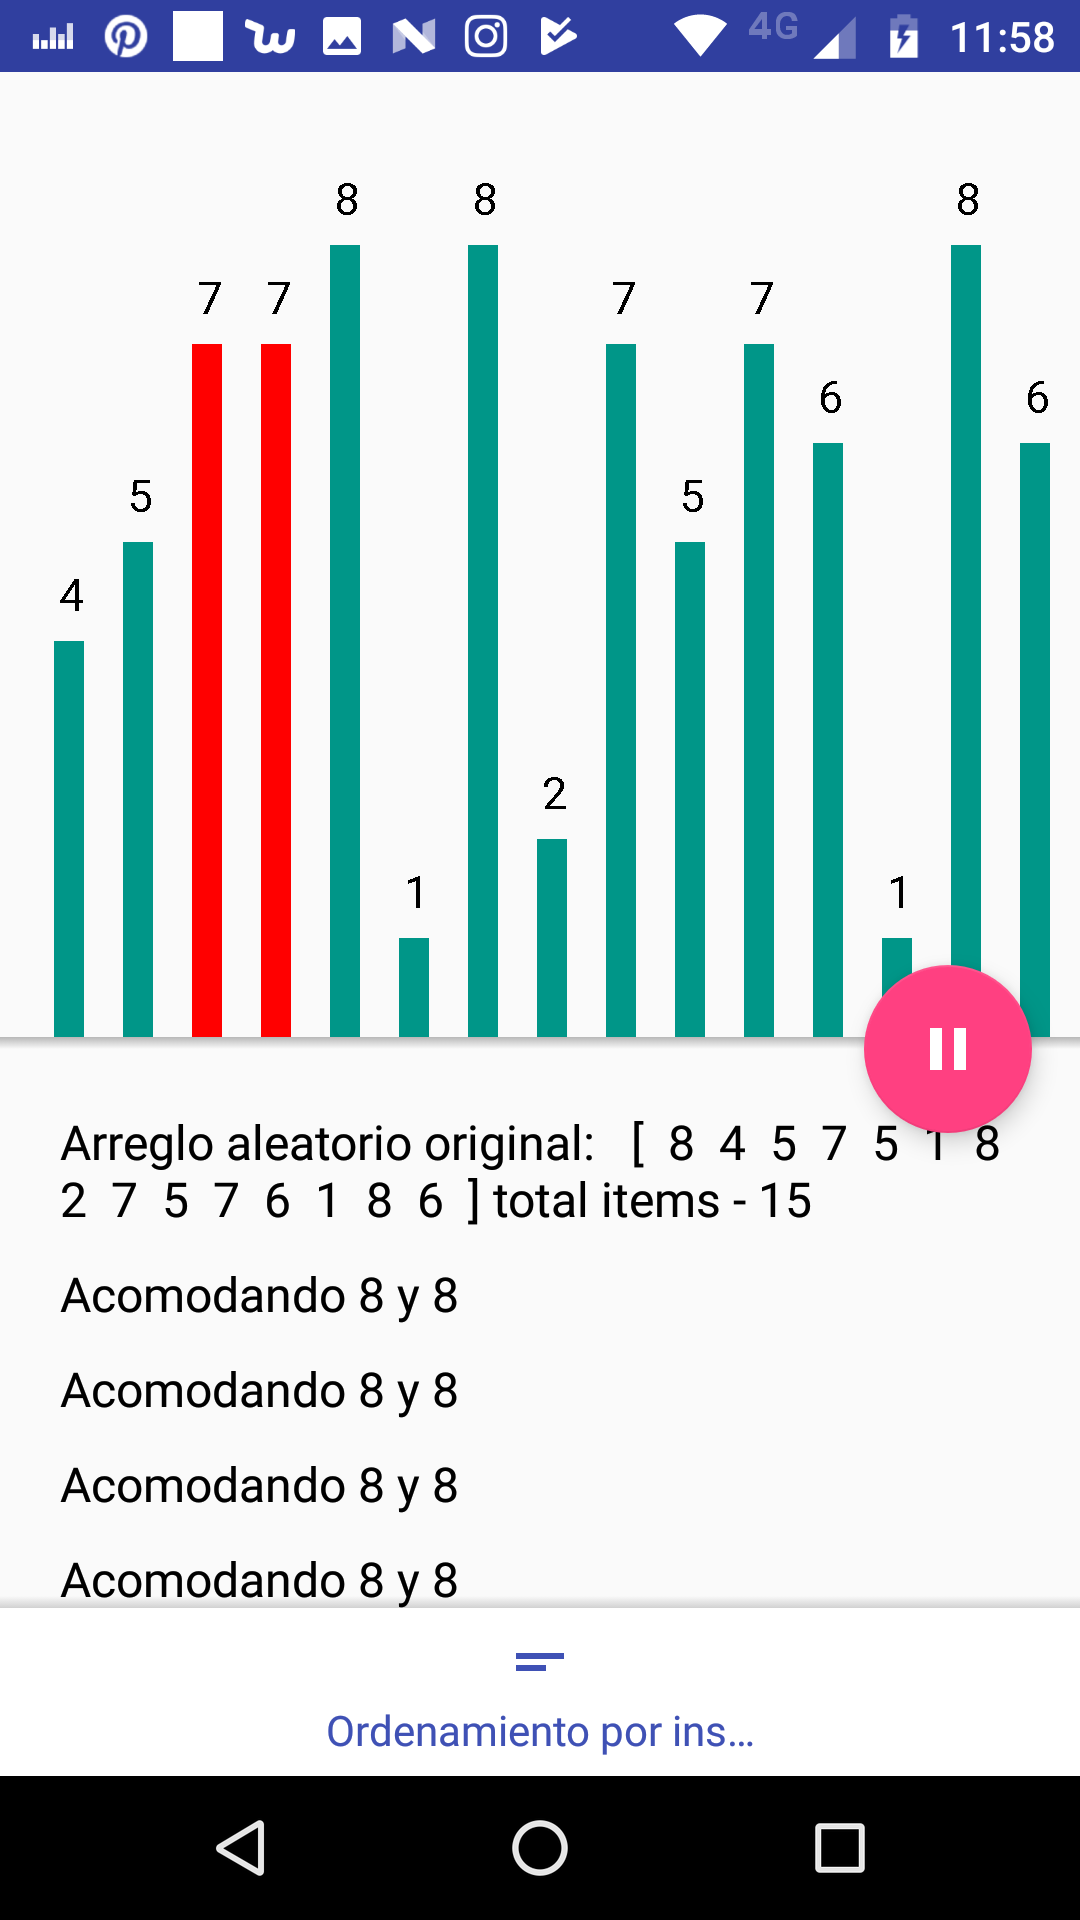
\includegraphics[width=2.3cm]{Plagio/Piratazo_Oscar1}\hspace{0.05cm}
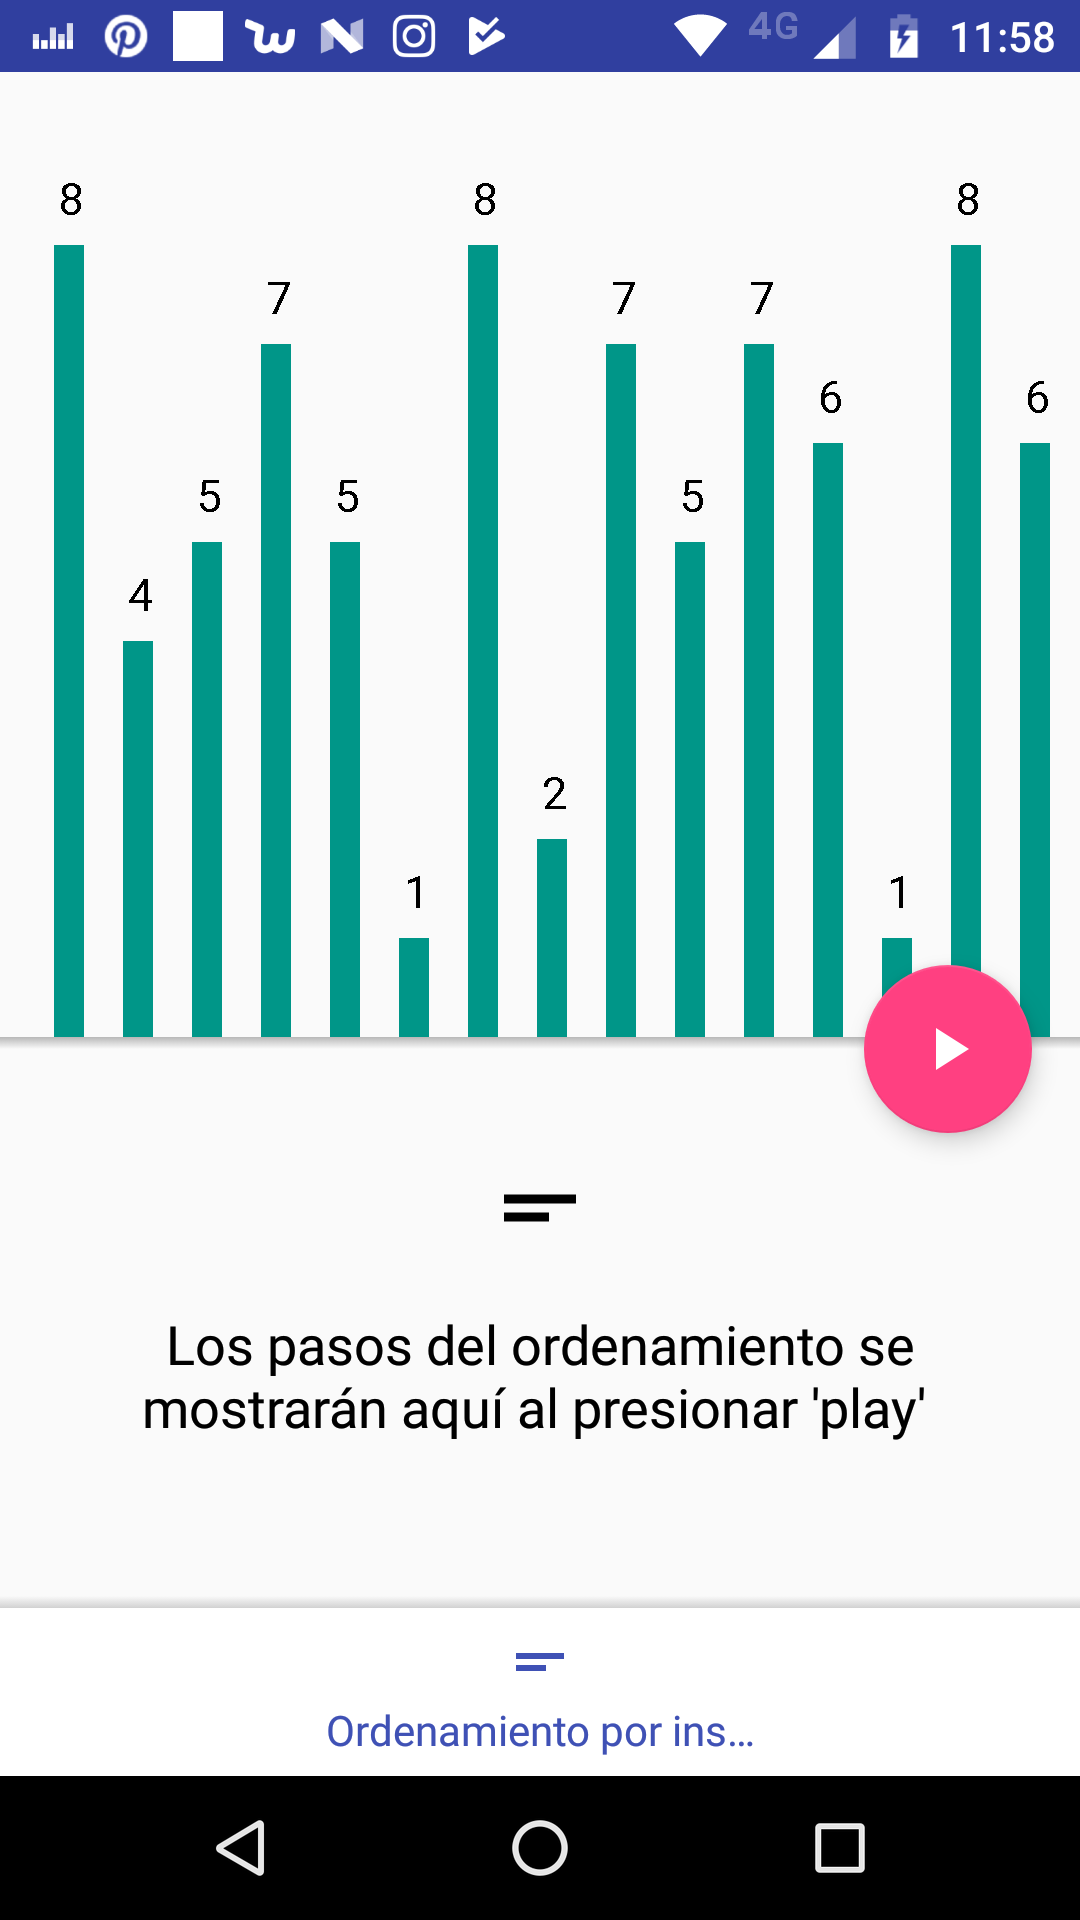
\includegraphics[width=2.3cm]{Plagio/Piratazo_Oscar2}\\
Proyecto ``clonado''
\end{center}	
\end{columns}
\end{frame}

